\documentclass[fleqn]{VUMIFKompMagistrinis}
\usepackage{algorithmicx}
\usepackage{algorithm}
\usepackage{algpseudocode}
\usepackage{amsfonts}
\usepackage{amsmath}
\usepackage{bm}
\usepackage{caption}
\usepackage{color}
\usepackage{float}
\usepackage{graphicx}
\usepackage{listings}
\usepackage{subfig}
\usepackage{wrapfig}

% Titulinio aprašas (nereikalingus elementus užkomentuoti)
\university{Vilniaus universitetas}
\faculty{Matematikos ir informatikos fakultetas}
\institute{Informatikos institutas}  % Užkomentavus šią eilutę - institutas neįtraukiamas į titulinį
\department{Kompiuterijos katedra}
\papertype{Magistro baigiamasis darbas}
\title{Nutolusios programinės įrangos instaliavimo ir administravimo sistemos}
\titleineng{Remote software installation and administration systems}
\author{Vardenis Pavardenis}
% \status{X kurso, Y grupės studentas}
% \secondauthor{Vardonis Pavardonis}   % Pridėti antrą autorių
% \thirdauthor{Vardonis Pavardonis}   % Pridėti antrą autorių
% \fourthauthor{Vardonis Pavardonis}   % Pridėti antrą autorių
\supervisor{prof. habil. dr. Vardaitis Pavardaitis}
%\reviewer{doc. dr. Vardauskas Pavardauskas}
\date{Vilnius \\ \the\year}

% Nustatymai
% \setmainfont{Palemonas}  % Pakeisti teksto šriftą į Palemonas (turi būti įdiegtas sistemoje)
\bibliography{bibliografija}  % Literatūros šaltinių aprašų failas bus bibliografija.bib

\begin{document}
\maketitle

\tableofcontents

\sectionnonum{Sutartinių terminų žodynas}
Sutartinių ženklų, simbolių, vienetų, trumpinimų ir terminų sąrašas sudaromas
tada, jei ženklų, simbolių, vienetų ir terminų bendras skaičius didesnis nei 10
ir kiekvienas iš jų tekste kartojasi daugiau nei 3 kartus. 

\santrauka{Santrauka}
Glaustai aprašomas darbo turinys: pristatomi darbo tikslai, analizuotos ir
tirtos problemos, atlikti eksperimentai bei padarytos išvados, gautos
rekomentacijos. Santraukos apimtis ne didesnė nei 0,5 puslapio. Santraukų gale
nurodomi darbo raktiniai žodžiai. 
% Nurodomi iki 5 svarbiausių temos raktinių žodžių (terminų).
% Vienas terminas gali susidėti iš kelių žodžių.
% \raktiniaizodziai{raktinis žodis 1, raktinis žodis 2, raktinis žodis 3, raktinis žodis 4, raktinis žodis 5}

\summary{Summary}
Santrauka anglų kalba. Santraukos apimtis ne didesnė nei 0,5 puslapio.
% \keywords{keyword 1, keyword 2, keyword 3, keyword 4, keyword 5}


\sectionnonum{Įvadas}
Įvade aprašomi darbo tikslai, nurodomas temos aktualumas, motyvacija,
formuluojamas sprendžiamas uždavinys ir siekiami/pasiekti rezultatai.
Aptariamos teorinės darbo prielaidos bei metodika, apibrėžiamas tiriamasis
objektas, apibūdinami su tema susiję literatūros ar kitokie šaltiniai, temos
analizės tvarka, darbo atlikimo aplinkybės, pateikiama žinių apie naudojamus
instrumentus (programas ir kt.).

\section{Pirmasis pagrindinės dalies skyrius}
Pagrindinėje dalyje aprašoma ir pagrindžiama viso darbo metodika, analizuojama
medžiaga, sukurtos sistemos/modeliai/metodikos/technologijos/algoritmai (toliau
vadinama - sistemomis*), jų įvertinimai, palyginimai, aprašomi pasiekti
rezultatai, detalios išvados. Priklausomai nuo darbo pobūdžio jame gali būti
šios dalys:
\begin{itemize}
    \item Motyvacija, bei susijusių darbų aprašymas - jei įvade nepilnai
        pagrįsta darbo motyvacija, ar pats darbas reikalauja tam tikrų
        susijusių darbų detalaus aprašymo.
    \item Analizės dalis - jei darbe lyginamos kelios sistemos*, šioje dalyje
        aprašoma atlikta analizė, palyginimai, įvertinimai.
    \item Kuriamos sistemos* detalus aprašymas, pagrindžiant kiekvieną žingsnį
        ar sugalvotą patobulinimą/naujovę, kodėl buvo priimti tokie sprendimai,
        kokiu rezultatų tikimasi.
    \item Atliktų eksperimentų/testų sąlygos, tikslingumas, ko buvo tikėtasi,
        kokie rezultatai gauti, padarytos išvados.
\end{itemize}

Šios dalys išvardintos kaip pavyzdys ir nebūtinai turi būti darbe, nes
kiekvieno darbo struktūra priklauso nuo nagrinėjamos temos, bei tyrimo
pobūdžio. Konkrečios darbo dalys turėtų būti suderintos su savo darbo vadovu.

\subsection{Poskyris}
Citavimo pavyzdžiai: cituojamas vienas šaltinis \cite{PvzStraipsnLt}; cituojami
keli šaltiniai \cite{PvzStraipsnEn, PvzKonfLt, PvzKonfEn, PvzKnygLt, PvzKnygEn,
PvzElPubLt, PvzElPubEn, PvzMagistrLt, PvzPhdEn}.

\subsubsection{Poskyrio poskyris}
\subsubsubsection{Trečio lygio poskyris}
\section{Antrasis skyrius}
\subsection{Poskyris}
\begin{equation}\label{eq:pavyzdys}
    y = \sum_{i=1}^N x_i
\end{equation}

\subsection{Poskyris}

\sectionnonum{Išvados ir rekomendacijos}
Išvadų ir rekomendacijų dalyje išdėstomi pagrindiniai darbo rezultatai (kažkas
išanalizuota, kažkas sukurta, kažkas įdiegta), pateikiamos išvados (daromi
nagrinėtų problemų sprendimo metodų palyginimai, siūlomos rekomendacijos,
akcentuojamos naujovės).

\sectionnonum{Ateities tyrimų planas}
Pristatomi ateities darbai ir/ar jų planas, gairės tolimesniems darbams....

\printbibliography[heading=bibintoc]  % Šaltinių sąraše abėcėlės tvarka išdėstomi darbe panaudotų
% (cituotų, perfrazuotų ar bent paminėtų) mokslo leidinių, kitokių publikacijų
% bibliografiniai aprašai. Aprašai pateikiami netransliteruoti.

\startappendix{Priedai}  % Priedai
Šiame skyriuje trumpai apibūdinama, kas pateikta kiekviename priede.

% Prieduose pateikiami programų tekstai, lentelės, schemos, paveiksliukai ir
% kita papildoma medžiaga, kuri yra papildanti darbo turinį. Jeigu lentelės,
% paveiksliukai yra nedideli ir jų nedaug, jie turi būti pateikti pagrindinėje
% dalyje.
\section{Pirmojo priedo pavadinimas}
Pirmojo priedo tekstas.
\begin{figure}[H]
    \centering
    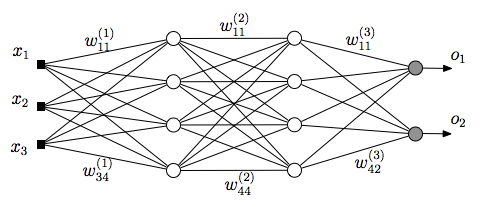
\includegraphics[scale=0.5]{img/MLP}
    \caption{Paveikslėlio pavyzdys}
    \label{img:mlp}
\end{figure}


\section{Antrojo priedo pavadinimas}
% tablesgenerator.com - converts calculators (e.g. excel) tables to LaTeX
\begin{table}[H]\footnotesize
  \centering
  \caption{Lentelės pavyzdys}
  \begin{tabular}{|l|c|c|} \hline
    Algoritmas    & $\bar{x}$ & $\sigma^{2}$ \\
    \hline
    Algoritmas A  & 1.6335    & 0.5584 \\
    Algoritmas B  & 1.7395    & 0.5647 \\
    \hline
  \end{tabular}
  \label{tab:table example}
\end{table}

\end{document}
